% ============================================================
% Ride-share adaptation to extreme weather (NYC, Hurricane Ida)
% Compiles at the repo root (locally and on Overleaf).
% Figures: output/fig/   Tables: output/reg/ (generated by R -- do not edit)
% ============================================================
\documentclass[12pt]{article}
\usepackage[margin=1in]{geometry}
\usepackage{graphicx,adjustbox,booktabs,amsmath,setspace,caption}
\usepackage[colorlinks=true,allcolors=blue]{hyperref}
\graphicspath{{output/fig/}}
\onehalfspacing

\title{Ride-share Adaptation to Extreme Weather: Hurricane Ida in NYC}
\author{EK}
\date{\today}

\begin{document}
\maketitle

\section{Descriptives}
\begin{figure}[ht]\centering
  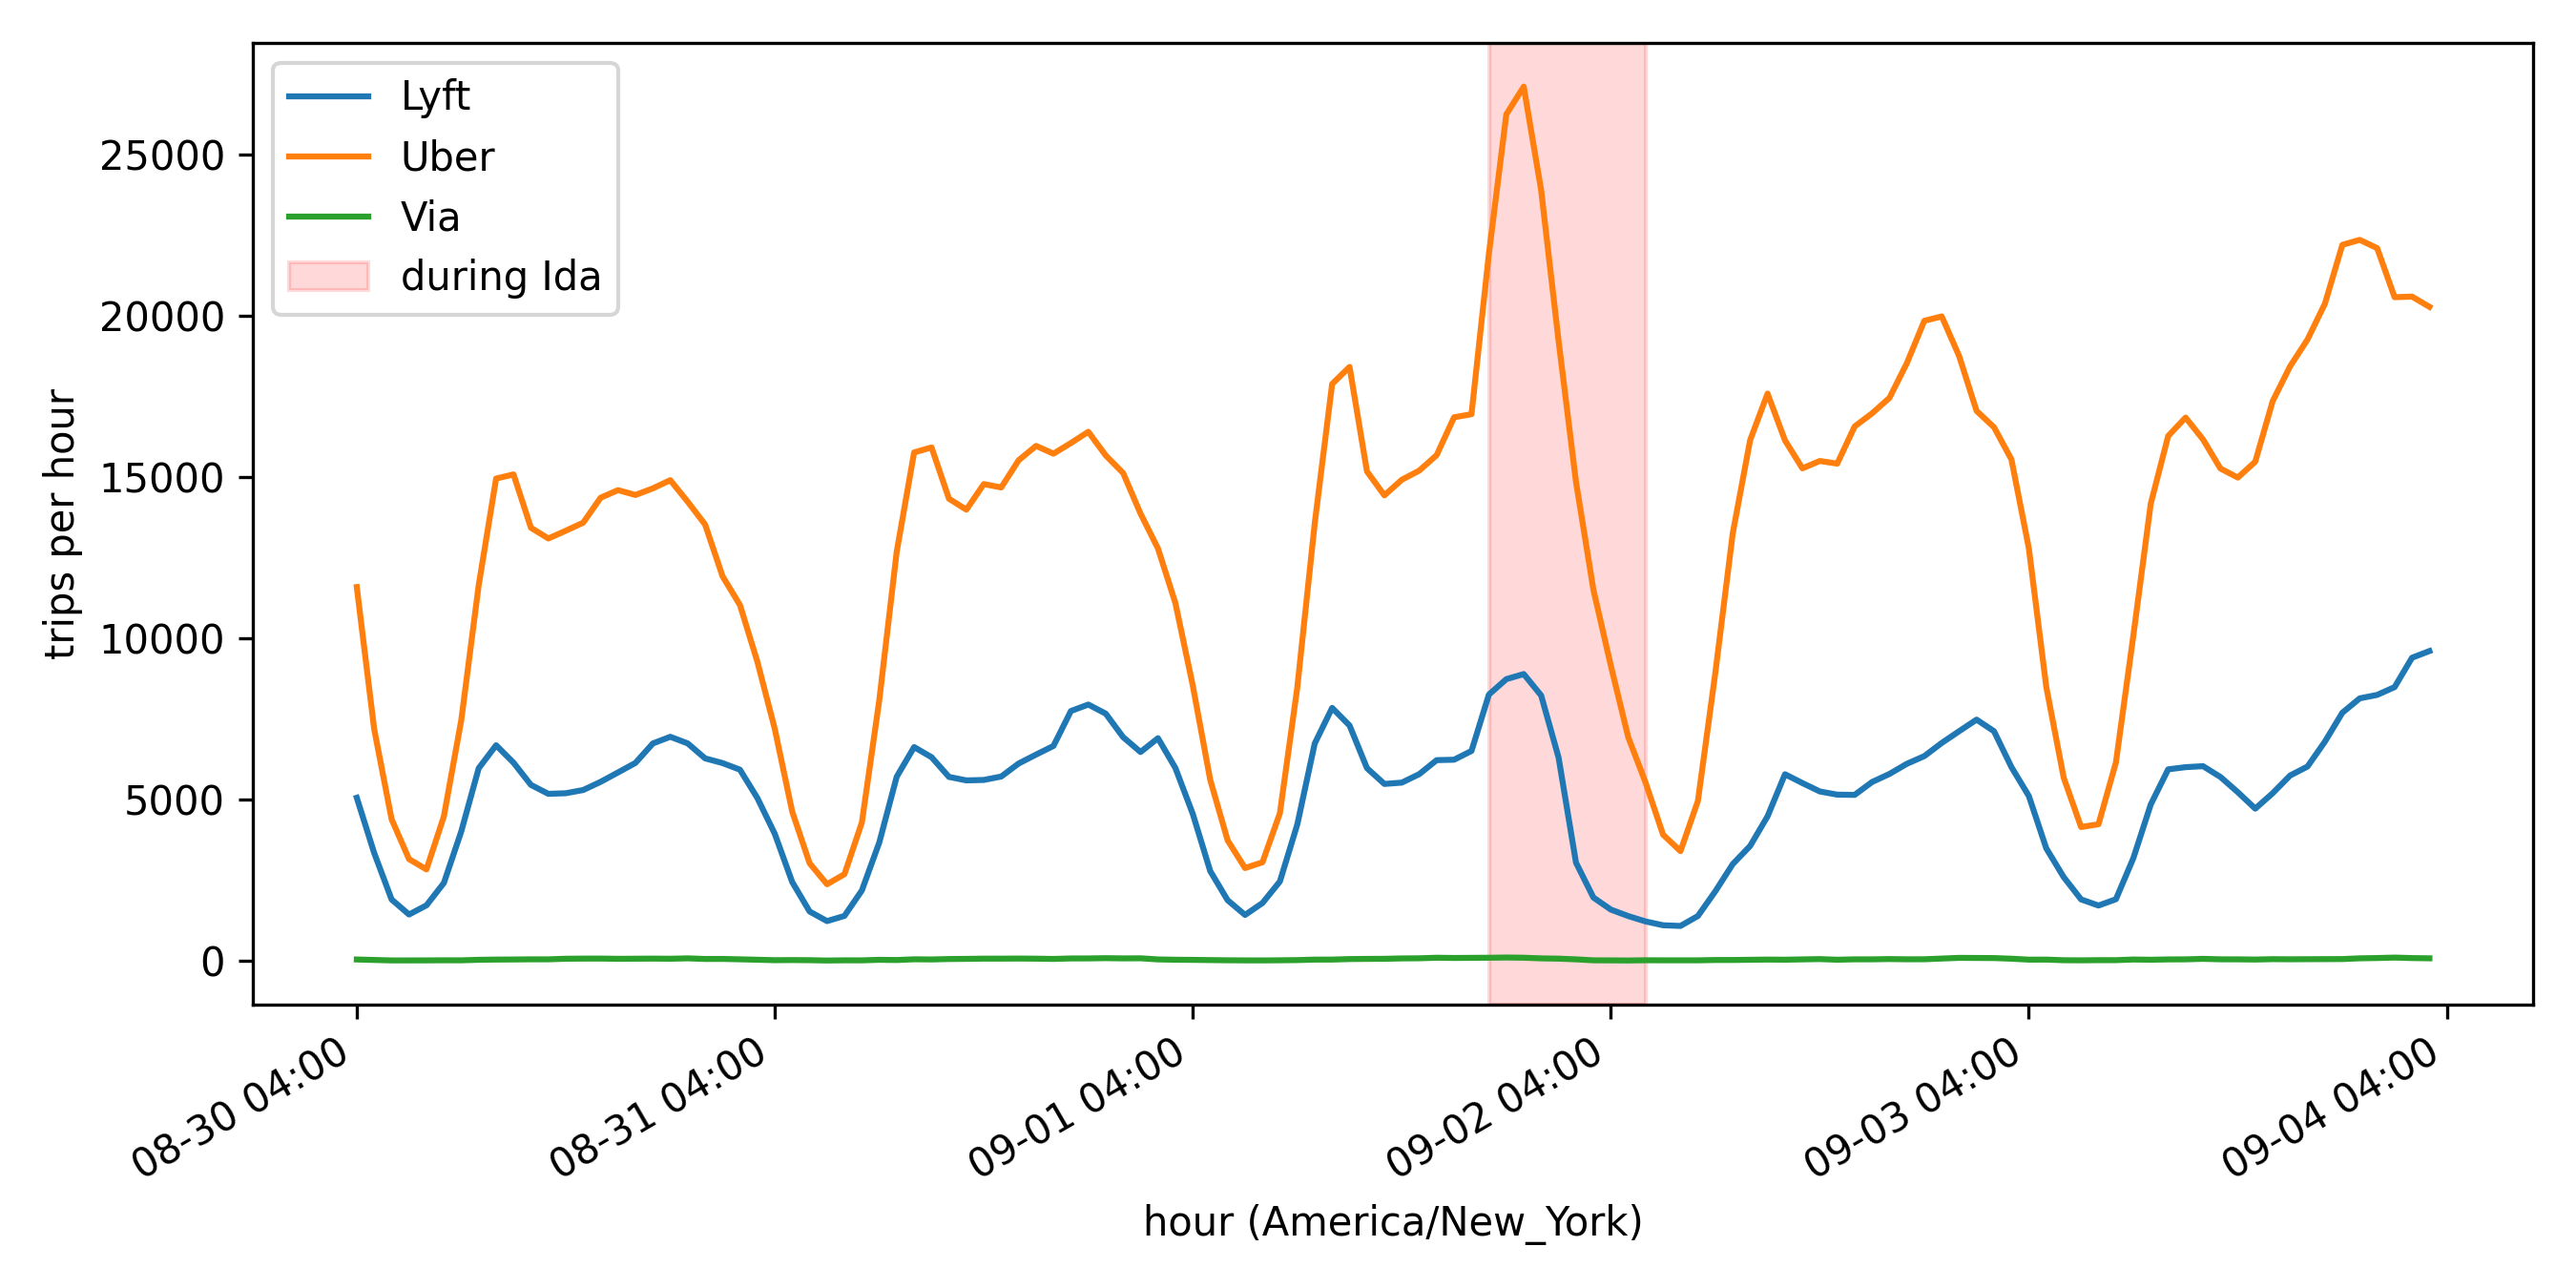
\includegraphics[width=\linewidth]{trips_hourly_ida_window.png}
  \caption{Hourly trips around Ida landfall.}
  \label{fig:trips_hourly}
\end{figure}

\section{Driver share and weather}
\begin{figure}[ht]\centering
  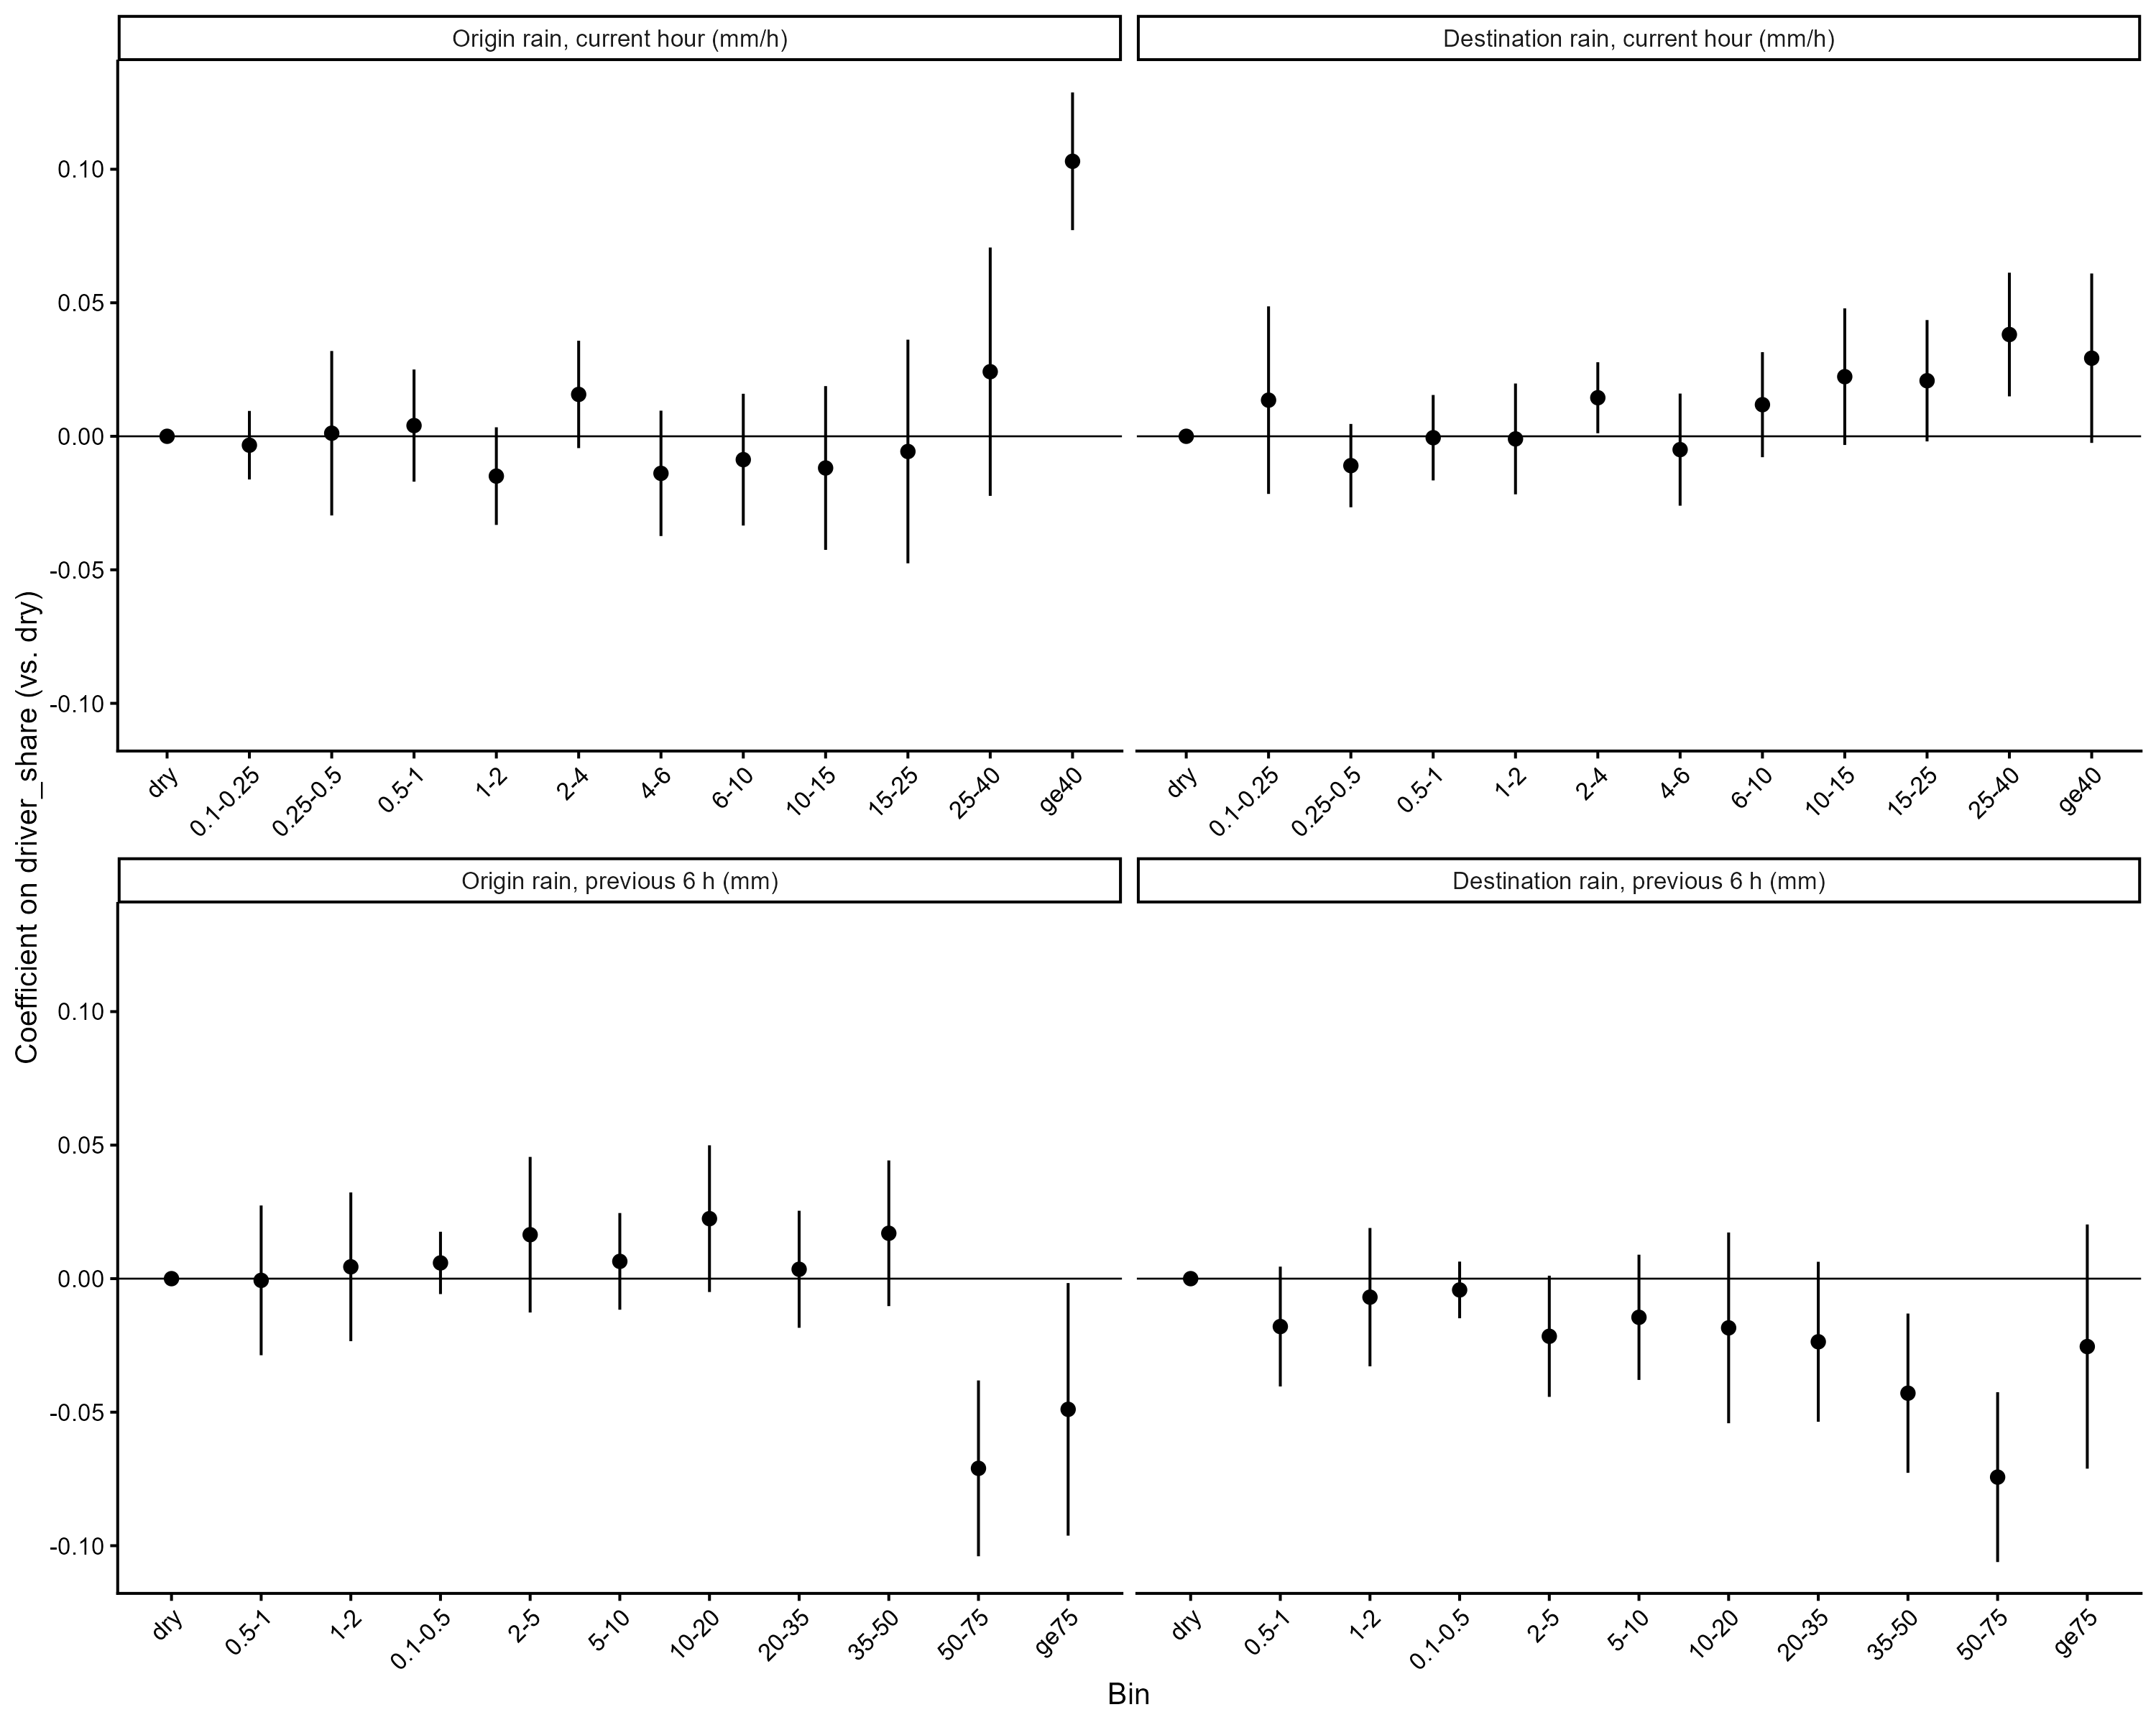
\includegraphics[width=\linewidth]{driver_share_weather_bins_augsep2021_r6.png}
  \caption{Driver share by rainfall bin, Aug--Sep 2021.}
  \label{fig:driver_share_bins}
\end{figure}

\begin{table}[ht]\centering
  \caption{Driver share by rainfall bin, Aug--Sep 2021}
  \label{tab:driver_share_bins}
  \ifdefined\ifclassloaded
\@ifclassloaded{beamer}{\begin{adjustbox}{max width=\linewidth}}{}
\fi

\begingroup
\centering
\begin{tabular}{lc}
   \tabularnewline \midrule \midrule
   Dependent Variable:                           & driver\_share\\   
   Sample:                                       & augsep2021\_r6 \\    
   Model:                                        & (1)\\  
   \midrule
   \emph{Variables}\\
   Origin rain, current hour (mm/h) $=$ 0.1-0.25 & -0.0033\\   
                                                 & (0.0065)\\   
   Origin rain, current hour (mm/h) $=$ 0.25-0.5 & 0.0011\\   
                                                 & (0.0157)\\   
   Origin rain, current hour (mm/h) $=$ 0.5-1    & 0.0040\\   
                                                 & (0.0107)\\   
   Origin rain, current hour (mm/h) $=$ 1-2      & -0.0149\\   
                                                 & (0.0093)\\   
   Origin rain, current hour (mm/h) $=$ 2-4      & 0.0157\\   
                                                 & (0.0103)\\   
   Origin rain, current hour (mm/h) $=$ 4-6      & -0.0139\\   
                                                 & (0.0120)\\   
   Origin rain, current hour (mm/h) $=$ 6-10     & -0.0087\\   
                                                 & (0.0126)\\   
   Origin rain, current hour (mm/h) $=$ 10-15    & -0.0119\\   
                                                 & (0.0156)\\   
   Origin rain, current hour (mm/h) $=$ 15-25    & -0.0057\\   
                                                 & (0.0214)\\   
   Origin rain, current hour (mm/h) $=$ 25-40    & 0.0242\\   
                                                 & (0.0237)\\   
   Origin rain, current hour (mm/h) $=$ ge40     & 0.1030$^{***}$\\   
                                                 & (0.0132)\\   
   Dest. rain, current hour (mm/h) $=$ 0.1-0.25  & 0.0135\\   
                                                 & (0.0179)\\   
   Dest. rain, current hour (mm/h) $=$ 0.25-0.5  & -0.0110\\   
                                                 & (0.0080)\\   
   Dest. rain, current hour (mm/h) $=$ 0.5-1     & -0.0005\\   
                                                 & (0.0082)\\   
   Dest. rain, current hour (mm/h) $=$ 1-2       & -0.0010\\   
                                                 & (0.0106)\\   
   Dest. rain, current hour (mm/h) $=$ 2-4       & 0.0144$^{**}$\\   
                                                 & (0.0068)\\   
   Dest. rain, current hour (mm/h) $=$ 4-6       & -0.0050\\   
                                                 & (0.0107)\\   
   Dest. rain, current hour (mm/h) $=$ 6-10      & 0.0118\\   
                                                 & (0.0100)\\   
   Dest. rain, current hour (mm/h) $=$ 10-15     & 0.0223$^{*}$\\   
                                                 & (0.0131)\\   
   Dest. rain, current hour (mm/h) $=$ 15-25     & 0.0208$^{*}$\\   
                                                 & (0.0116)\\   
   Dest. rain, current hour (mm/h) $=$ 25-40     & 0.0381$^{***}$\\   
                                                 & (0.0118)\\   
   Dest. rain, current hour (mm/h) $=$ ge40      & 0.0293$^{*}$\\   
                                                 & (0.0162)\\   
   Origin rain, prev. 6 h (mm) $=$ 0.1-0.5       & 0.0059\\   
                                                 & (0.0060)\\   
   Origin rain, prev. 6 h (mm) $=$ 0.5-1         & -0.0006\\   
                                                 & (0.0143)\\   
   Origin rain, prev. 6 h (mm) $=$ 1-2           & 0.0044\\   
                                                 & (0.0142)\\   
   Origin rain, prev. 6 h (mm) $=$ 2-5           & 0.0165\\   
                                                 & (0.0149)\\   
   Origin rain, prev. 6 h (mm) $=$ 5-10          & 0.0065\\   
                                                 & (0.0092)\\   
   Origin rain, prev. 6 h (mm) $=$ 10-20         & 0.0225\\   
                                                 & (0.0140)\\   
   Origin rain, prev. 6 h (mm) $=$ 20-35         & 0.0035\\   
                                                 & (0.0112)\\   
   Origin rain, prev. 6 h (mm) $=$ 35-50         & 0.0170\\   
                                                 & (0.0139)\\   
   Origin rain, prev. 6 h (mm) $=$ 50-75         & -0.0710$^{***}$\\   
                                                 & (0.0168)\\   
   Origin rain, prev. 6 h (mm) $=$ ge75          & -0.0489$^{**}$\\   
                                                 & (0.0241)\\   
   Dest. rain, prev. 6 h (mm) $=$ 0.1-0.5        & -0.0042\\   
                                                 & (0.0054)\\   
   Dest. rain, prev. 6 h (mm) $=$ 0.5-1          & -0.0179\\   
                                                 & (0.0114)\\   
   Dest. rain, prev. 6 h (mm) $=$ 1-2            & -0.0069\\   
                                                 & (0.0132)\\   
   Dest. rain, prev. 6 h (mm) $=$ 2-5            & -0.0216$^{*}$\\   
                                                 & (0.0116)\\   
   Dest. rain, prev. 6 h (mm) $=$ 5-10           & -0.0145\\   
                                                 & (0.0120)\\   
   Dest. rain, prev. 6 h (mm) $=$ 10-20          & -0.0184\\   
                                                 & (0.0182)\\   
   Dest. rain, prev. 6 h (mm) $=$ 20-35          & -0.0236\\   
                                                 & (0.0153)\\   
   Dest. rain, prev. 6 h (mm) $=$ 35-50          & -0.0429$^{***}$\\   
                                                 & (0.0152)\\   
   Dest. rain, prev. 6 h (mm) $=$ 50-75          & -0.0743$^{***}$\\   
                                                 & (0.0162)\\   
   Dest. rain, prev. 6 h (mm) $=$ ge75           & -0.0254\\   
                                                 & (0.0233)\\   
   \midrule
   \emph{Fixed-effects}\\
   platform                                      & Yes\\  
   pu\_fe                                        & Yes\\  
   do\_fe                                        & Yes\\  
   month                                         & Yes\\  
   dow                                           & Yes\\  
   \midrule
   \emph{Fit statistics}\\
   Observations                                  & 18,109,320\\  
   R$^2$                                         & 0.00140\\  
   \midrule \midrule
   \multicolumn{2}{l}{\emph{Clustered (pu\_zone\_id \& date\_int) standard-errors in parentheses}}\\
   \multicolumn{2}{l}{\emph{Signif. Codes: ***: 0.01, **: 0.05, *: 0.1}}\\
\end{tabular}
 
\par \raggedright 
Dependent variable: driver\_share = driver\_pay / base\_passenger\_fare (trip level, cell mean). Current-hour rain bins (mm/h, left-closed) at origin (pickup hour) and destination (dropoff hour); reference bin is dry, below 0.1 mm/h. Previous-6-hour rain bins (mm, left-closed): total rain in hours t-6 to t-1 before the pickup (origin) or dropoff (destination) hour, excluding the current hour, requiring at least 5 of the 6 hours observed; reference bin is dry, below 0.1 mm. No temperature controls. Trips ending outside NYC (zone 265) are kept; their destination-rain indicators are absorbed by the destination-zone x hour FE, so they inform only origin-rain coefficients. Standard errors two-way clustered by pickup taxi zone and pickup date. Observations are OD cells (platform x PU zone x DO zone x pickup hour x dropoff hour) weighted by trips per cell, so estimates equal trip-level OLS. Fixed effects: platform, PU zone x pickup hour-of-day, DO zone x dropoff hour-of-day, month, day-of-week. No date fixed effect: identification includes variation across days within a month as well as across zones and hours. Access-a-Ride trips excluded. Significance: *** p<0.01, ** p<0.05, * p<0.1. N cells = 18,109,352; N trips = 28,774,232; months = 8,9.
\par\endgroup


\ifdefined\ifclassloaded
\@ifclassloaded{beamer}{\end{adjustbox}}{}
\fi

\end{table}

\section{Driver share and weather: full-year 2021}
\begin{figure}[ht]\centering
  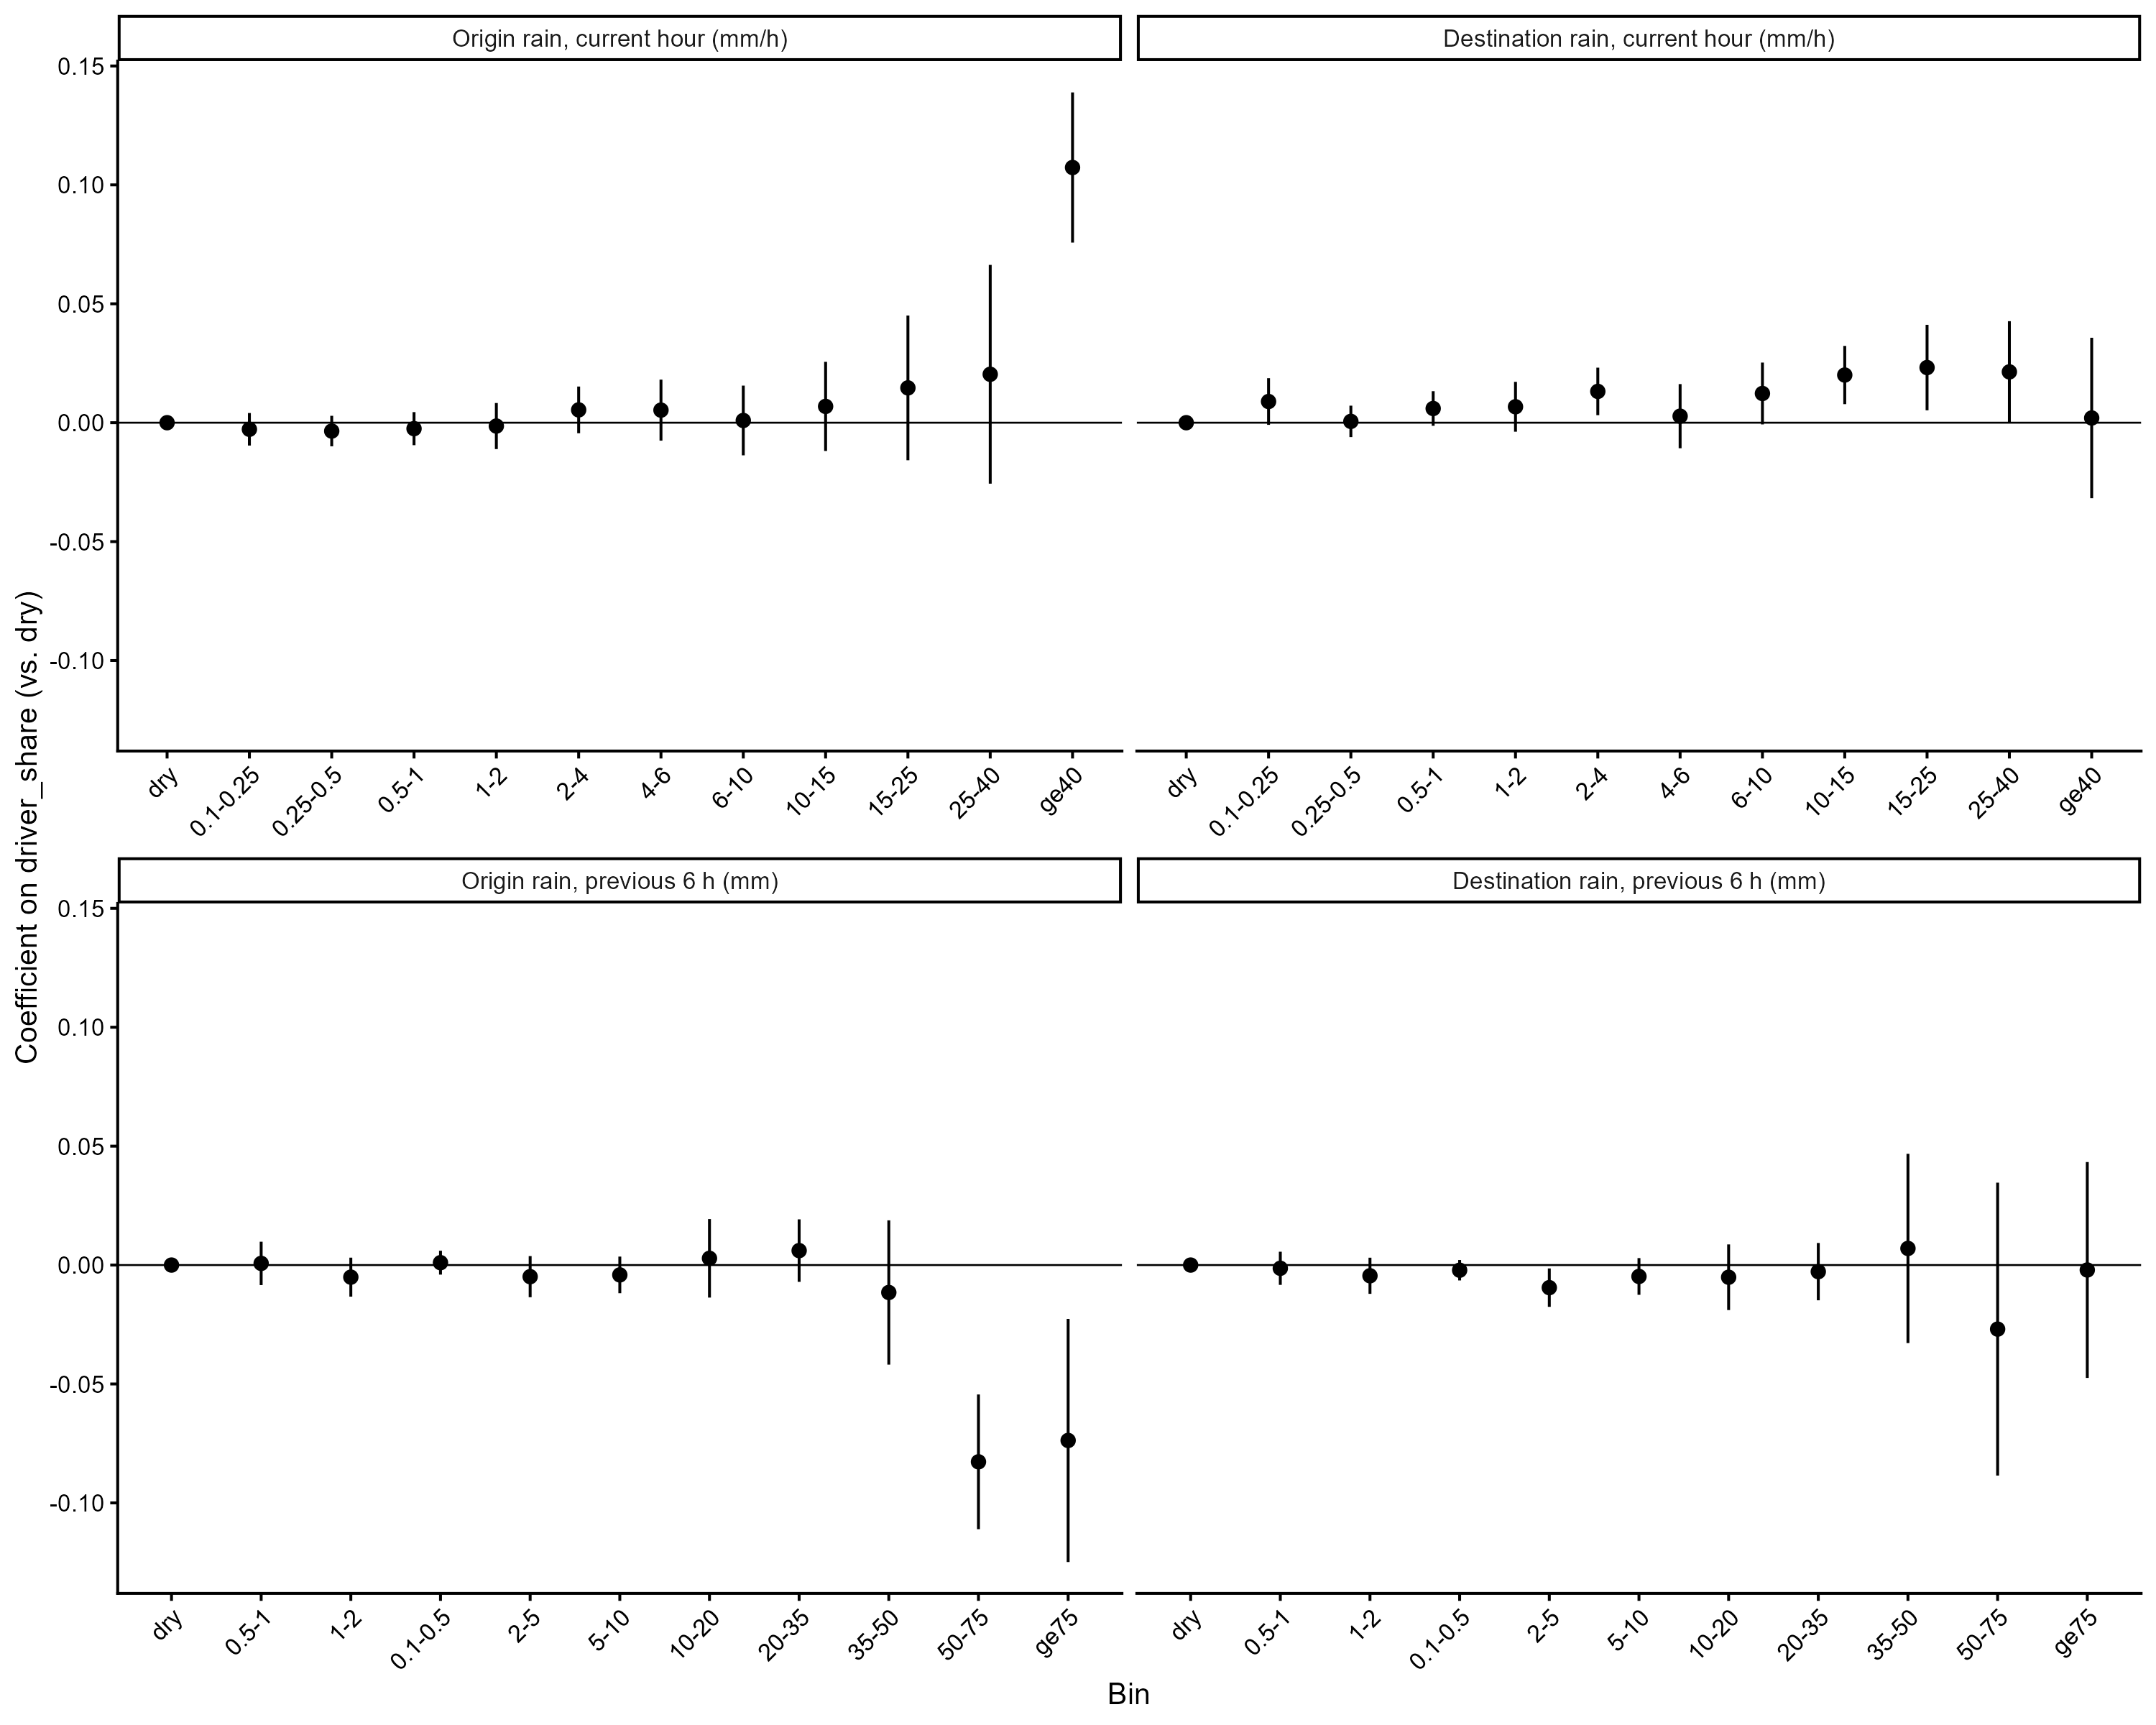
\includegraphics[width=\linewidth]{driver_share_weather_bins_2021.png}
  \caption{Driver share by rainfall bin, full-year 2021.}
  \label{fig:driver_share_bins_2021}
\end{figure}

\begin{table}[ht]\centering
  \caption{Driver share by rainfall bin, full-year 2021}
  \label{tab:driver_share_bins_2021}
  \ifdefined\ifclassloaded
\@ifclassloaded{beamer}{\begin{adjustbox}{max width=\linewidth}}{}
\fi
\begingroup
\centering
\begin{tabular}{lc}
   \tabularnewline \midrule \midrule
   Dependent Variable: & driver\_share\\
   Sample: & 2021 \\
   Model: & (1)\\
   \midrule
   \emph{Variables}\\
   Origin rain, current hour (mm/h) $=$ 0.1-0.25 & -0.0028\\
    & (0.0035)\\
   Origin rain, current hour (mm/h) $=$ 0.25-0.5 & -0.0035\\
    & (0.0033)\\
   Origin rain, current hour (mm/h) $=$ 0.5-1 & -0.0025\\
    & (0.0035)\\
   Origin rain, current hour (mm/h) $=$ 1-2 & -0.0014\\
    & (0.0049)\\
   Origin rain, current hour (mm/h) $=$ 2-4 & 0.0054\\
    & (0.0050)\\
   Origin rain, current hour (mm/h) $=$ 4-6 & 0.0053\\
    & (0.0065)\\
   Origin rain, current hour (mm/h) $=$ 6-10 & 0.0009\\
    & (0.0075)\\
   Origin rain, current hour (mm/h) $=$ 10-15 & 0.0069\\
    & (0.0096)\\
   Origin rain, current hour (mm/h) $=$ 15-25 & 0.0146\\
    & (0.0155)\\
   Origin rain, current hour (mm/h) $=$ 25-40 & 0.0204\\
    & (0.0235)\\
   Origin rain, current hour (mm/h) $=$ ge40 & 0.1073$^{***}$\\
    & (0.0161)\\
   Dest. rain, current hour (mm/h) $=$ 0.1-0.25 & 0.0089$^{*}$\\
    & (0.0050)\\
   Dest. rain, current hour (mm/h) $=$ 0.25-0.5 & 0.0006\\
    & (0.0034)\\
   Dest. rain, current hour (mm/h) $=$ 0.5-1 & 0.0060\\
    & (0.0037)\\
   Dest. rain, current hour (mm/h) $=$ 1-2 & 0.0067\\
    & (0.0053)\\
   Dest. rain, current hour (mm/h) $=$ 2-4 & 0.0132$^{**}$\\
    & (0.0051)\\
   Dest. rain, current hour (mm/h) $=$ 4-6 & 0.0027\\
    & (0.0069)\\
   Dest. rain, current hour (mm/h) $=$ 6-10 & 0.0123$^{*}$\\
    & (0.0066)\\
   Dest. rain, current hour (mm/h) $=$ 10-15 & 0.0200$^{***}$\\
    & (0.0062)\\
   Dest. rain, current hour (mm/h) $=$ 15-25 & 0.0232$^{**}$\\
    & (0.0092)\\
   Dest. rain, current hour (mm/h) $=$ 25-40 & 0.0214$^{*}$\\
    & (0.0109)\\
   Dest. rain, current hour (mm/h) $=$ ge40 & 0.0020\\
    & (0.0172)\\
   Origin rain, prev. 6 h (mm) $=$ 0.1-0.5 & 0.0010\\
    & (0.0026)\\
   Origin rain, prev. 6 h (mm) $=$ 0.5-1 & 0.0007\\
    & (0.0047)\\
   Origin rain, prev. 6 h (mm) $=$ 1-2 & -0.0051\\
    & (0.0042)\\
   Origin rain, prev. 6 h (mm) $=$ 2-5 & -0.0049\\
    & (0.0044)\\
   Origin rain, prev. 6 h (mm) $=$ 5-10 & -0.0041\\
    & (0.0039)\\
   Origin rain, prev. 6 h (mm) $=$ 10-20 & 0.0028\\
    & (0.0084)\\
   Origin rain, prev. 6 h (mm) $=$ 20-35 & 0.0061\\
    & (0.0067)\\
   Origin rain, prev. 6 h (mm) $=$ 35-50 & -0.0115\\
    & (0.0155)\\
   Origin rain, prev. 6 h (mm) $=$ 50-75 & -0.0827$^{***}$\\
    & (0.0145)\\
   Origin rain, prev. 6 h (mm) $=$ ge75 & -0.0738$^{***}$\\
    & (0.0261)\\
   Dest. rain, prev. 6 h (mm) $=$ 0.1-0.5 & -0.0022\\
    & (0.0022)\\
   Dest. rain, prev. 6 h (mm) $=$ 0.5-1 & -0.0014\\
    & (0.0036)\\
   Dest. rain, prev. 6 h (mm) $=$ 1-2 & -0.0045\\
    & (0.0039)\\
   Dest. rain, prev. 6 h (mm) $=$ 2-5 & -0.0095$^{**}$\\
    & (0.0041)\\
   Dest. rain, prev. 6 h (mm) $=$ 5-10 & -0.0048\\
    & (0.0039)\\
   Dest. rain, prev. 6 h (mm) $=$ 10-20 & -0.0051\\
    & (0.0070)\\
   Dest. rain, prev. 6 h (mm) $=$ 20-35 & -0.0028\\
    & (0.0061)\\
   Dest. rain, prev. 6 h (mm) $=$ 35-50 & 0.0070\\
    & (0.0203)\\
   Dest. rain, prev. 6 h (mm) $=$ 50-75 & -0.0269\\
    & (0.0314)\\
   Dest. rain, prev. 6 h (mm) $=$ ge75 & -0.0021\\
    & (0.0232)\\
   \midrule
   \emph{Fixed-effects}\\
   platform & Yes\\
   pu\_fe & Yes\\
   do\_fe & Yes\\
   month & Yes\\
   dow & Yes\\
   \midrule
   \emph{Fit statistics}\\
   Observations & 106,438,465\\
   R$^2$ & 0.00080\\
   \midrule \midrule
   \multicolumn{2}{l}{\emph{Clustered (pu\_zone\_id \& date\_int) standard-errors in parentheses}}\\
   \multicolumn{2}{l}{\emph{Signif. Codes: ***: 0.01, **: 0.05, *: 0.1}}\\
\end{tabular}
 
\par \raggedright 
Dependent variable: driver\_share = driver\_pay / base\_passenger\_fare (trip level, cell mean). Current-hour rain bins (mm/h, left-closed) at origin (pickup hour) and destination (dropoff hour); reference bin is dry, below 0.1 mm/h. Previous-6-hour rain bins (mm, left-closed): total rain in hours t-6 to t-1 before the pickup (origin) or dropoff (destination) hour, excluding the current hour, requiring at least 5 of the 6 hours observed; reference bin is dry, below 0.1 mm. No temperature controls. Trips ending outside NYC (zone 265) are kept; their destination-rain indicators are absorbed by the destination-zone x hour FE, so they inform only origin-rain coefficients. Standard errors two-way clustered by pickup taxi zone and pickup date. Observations are OD cells (platform x PU zone x DO zone x pickup hour x dropoff hour) weighted by trips per cell, so estimates equal trip-level OLS. Fixed effects: platform, PU zone x pickup hour-of-day, DO zone x dropoff hour-of-day, month, day-of-week. No date fixed effect: identification includes variation across days within a month as well as across zones and hours. Access-a-Ride trips excluded. Significance: *** p<0.01, ** p<0.05, * p<0.1. N cells = 106,438,499; N trips = 171,429,675; months = 1,2,3,4,5,6,7,8,9,10,11,12. Estimated by exact batched FWL; validated against fixest::feols on Aug-Sep 2021 to 1e-6.
\par\endgroup
\ifdefined\ifclassloaded
\@ifclassloaded{beamer}{\end{adjustbox}}{}
\fi

\end{table}

\end{document}
